%%%%% Beginning of preamble %%%%%

\documentclass[12pt]{article}  %What kind of document (article) and what size
\usepackage[document]{ragged2e}

\usepackage{wrapfig}
%Packages to load which give you useful commands
\usepackage{graphicx}
\usepackage{amssymb, amsmath, amsthm}
\usepackage{fancyhdr}
\usepackage{tikz}
\usetikzlibrary{automata,positioning}
\usepackage[linguistics]{forest}
\usepackage{enumerate}
\usepackage{blkarray}
\usepackage[margin=1in]{geometry} 
\pagestyle{fancy}
\fancyhf{}
\lhead{MA 583: HW6, \today, Discussion A4}
\rhead{Benjamin Draves}


\renewcommand{\headrulewidth}{.4pt}
\renewcommand{\footrulewidth}{0.4pt}

\topmargin = -0.4 in
%\headheight = 0.0 in t
%\headsep = .3 in
\parskip = 0.2in
%\parindent = 0.0in

%%%%%%%%%%new commands%%%%%%%%%%%%
\newcommand{\N}{{\mathbb{N}}}
\newcommand{\Z}{{\mathbb{Z}}}
\newcommand{\R}{{\mathbb{R}}}
\newcommand{\Q}{{\mathbb{Q}}}
\newcommand{\e}{{\epsilon}}
\newcommand{\del}{{\delta}}
\newcommand{\m}{{\mid}}
\newcommand{\infsum}{{\sum_{n=1}^\infty}}
\newcommand{\la}{{\langle}}
\newcommand{\ra}{{\rangle}}
\newcommand{\E}{{\mathbb{E}}}
\newcommand{\V}{{\text{Var}}}
\newcommand{\prob}{{\mathbb{P}}}
\newcommand{\ind}{{\mathbf{1}}}

%defines a few theorem-type environments
\newtheorem{theorem}{Theorem}
\newtheorem{corollary}[theorem]{Corollary}
\newtheorem{definition}{Definition}
\newtheorem{lemma}[theorem]{Lemma}
%%%%% End of preamble %%%%%

\begin{document}

\begin{description}
\item[Exercise 4.3.1] This Markov Chain can be described by the following diagram. 

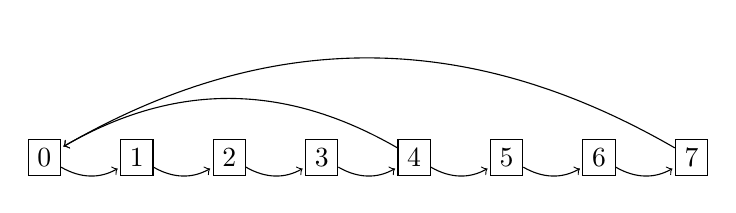
\begin{tikzpicture}[node distance=0.75cm]
% nodes
\node [draw] (0) {0};
\node [draw, right=of 0] (1) {1};
\node [draw, right=of 1] (2) {2};
\node [draw, right=of 2] (3) {3};
\node [draw, right=of 3] (4) {4};
\node [draw, right=of 4] (5) {5};
\node [draw, right=of 5] (6) {6};
\node [draw, right=of 6] (7) {7};
% arrows
\draw [every loop] 
	(0) edge[bend right] node{} (1)
	(1) edge[bend right] node{} (2)
	(2) edge[bend right] node{} (3)
	(3) edge[bend right] node{} (4)
	(4) edge[bend right] node{} (5)
	(5) edge[bend right] node{} (6)
	(6) edge[bend right] node{} (7)
	(4) edge[bend right] node{} (0)
	(7) edge[bend right] node{} (0); 
\end{tikzpicture}

Here, we see that every state communicates and hence their is only one equivalence class $\{0,1,\ldots, 7\}$. Therefore, any class property (e.g. periodicity) applies to the entire Markov Chain. Starting at state $0$, we see we can return in $5$ steps corresponding to $0\to1\to2\to3\to4\to0$ and 8 steps corresponding to $0\to1\to\dots\to7\to0$. Hence $$\{n\leq 20: P_{00}^{(n)}>0\} = \{5,8,10,13,15,16,18,20\}$$
Note that for $n\geq 40$ we have $P_{00}^{(n)}>0$. So for $n = 41$ and $n=43$, say (both primes), we have $gcd(41,43) = 1$. As $41,43\in\{n\in\N:P_{00}^{(n)}>0\}$ we see that the period of this state is $d(0)=1$. As there is only one communication class, this Markov Chain is aperiodic. 

\item[Exercise 4.3.2] Recall that we need only consider the sum $\sum_{n=1}^{\infty}P_{ii}^{(n)}$ to classify states as either recurrent or transient. First note that we can decompose this Markov Chain's state space $S$ into its communication classes as $S = \{0\}\cup\{1\}\cup\{2,4\}\cup\{3\}\cup\{5\}$. As transient/recurrent are class properties, we need only compute the above quantity for one state in each class. 
\begin{itemize}
\item State $0$: $\sum_{n=1}^{\infty}P_{00}^{(n)} = \sum_{n=1}^{\infty} (1/3)^n = 3/2 - 1 = 1/2<\infty$ \textbf{Transient}
\item State $1$: $\sum_{n=1}^{\infty}P_{11}^{(n)} = \sum_{n=1}^{\infty} (1/4)^n = 4/3 - 1 = 1/3<\infty$ \textbf{Transient}
\item State $2$: $\sum_{n=1}^{\infty}P_{22}^{(n)} = \sum_{n=1}^{\infty} (1)^{2n} = \infty$ \textbf{Recurrent}
\item State $3$: $\sum_{n=1}^{\infty}P_{33}^{(n)} = \sum_{n=1}^{\infty} 0 = 0$ \textbf{Transient}
\item State $5$: $\sum_{n=1}^{\infty}P_{55}^{(n)} = \sum_{n=1}^{\infty} (1) = \infty$ \textbf{Recurrent}
\end{itemize}
Hence, we see that $\{0,1,3\}$ are transient states and $\{2,4,5\}$ are recurrent states. 

\item[Problem 4.3.2] First recall that if a Markov Chain is irreducible then all its states must communicate by definition. That is for each $(i,j)$ there exists $k_{(i,j)}\in\N$ such that $P_{ij}^{k_{ij}}>0$. Let $k = \max_{(i,j)\in S\times S} k_{ij}$. We know that $k<\infty$ as it is a maximum over a finite set of finite elements. This then implies that$P_{ij}^{k}>0$ for all $i,j\in S$. That is, $P$ is regular. 

Again, since all states communicate, there is only one communication class. As a result, we need only show that there exists $j\in S$ such that $j$ is recurrent. Well, with $|S| = m$ we can write 
\begin{align*}
\sum_{j=1}^{m}P_{ij}^{n} &= 1\\
\sum_{n=1}^{\infty}\sum_{j=1}^{m}P_{ij}^{n} &= \infty\\
\sum_{j=1}^{m}\sum_{n=1}^{\infty}P_{ij}^{n} &= \infty\\
\end{align*}
Note we can change the order of summation as it is a finite sum of positive elements. As this is a finite sum, there exists $j*$ such that $\sum_{n=1}^{\infty}P_{ij*}^{n} = \infty$. With this in mind, we can also condition on the arrival of the chain to state $j*$ as follows
\begin{align*}
\infty = \sum_{n=1}^{\infty}P_{ij*}^{n} = \sum_{n=1}^{\infty}\sum_{m=1}^n P_{j*j*}^{(n-m)}f_{ij*}^{(m)} = \sum_{m=1}^{\infty}f_{ij*}^{(m)}\sum_{n=m}^{\infty} P_{j*j*}^{(n)}
\end{align*}
Now, notice that $\sum_{m=1}^{\infty}f_{ij*}^{(m)}$ is just the probability of going $i\to j*$ or $f_{ij*}$. Moreover, we know that $f_{ij*}\leq 1$ hence 
\begin{align*}
\infty = \sum_{m=1}^{\infty}f_{ij*}^{(m)}\sum_{n=m}^{\infty} P_{j*j*}^{(n)} = f_{ij*}\sum_{n=1}^{\infty} P_{j*j*}^{(n)} 
\end{align*}
Therefore, we see that $\sum_{n=1}^{\infty} P_{j*j*}^{(n)} = \infty$ and $j*$ is recurrent. As $j*$ is recurrent, so are all states in $S$. Therefore this aperiodic, irreducible Markov Chain is recurrent. 

\end{description}	
\end{document} 


